\documentclass[1p]{elsarticle_modified}
%\bibliographystyle{elsarticle-num}

%\usepackage[colorlinks]{hyperref}
%\usepackage{abbrmath_seonhwa} %\Abb, \Ascr, \Acal ,\Abf, \Afrak
\usepackage{amsfonts}
\usepackage{amssymb}
\usepackage{amsmath}
\usepackage{amsthm}
\usepackage{scalefnt}
\usepackage{amsbsy}
\usepackage{kotex}
\usepackage{caption}
\usepackage{subfig}
\usepackage{color}
\usepackage{graphicx}
\usepackage{xcolor} %% white, black, red, green, blue, cyan, magenta, yellow
\usepackage{float}
\usepackage{setspace}
\usepackage{hyperref}

\usepackage{tikz}
\usetikzlibrary{arrows}

\usepackage{multirow}
\usepackage{array} % fixed length table
\usepackage{hhline}

%%%%%%%%%%%%%%%%%%%%%
\makeatletter
\renewcommand*\env@matrix[1][\arraystretch]{%
	\edef\arraystretch{#1}%
	\hskip -\arraycolsep
	\let\@ifnextchar\new@ifnextchar
	\array{*\c@MaxMatrixCols c}}
\makeatother %https://tex.stackexchange.com/questions/14071/how-can-i-increase-the-line-spacing-in-a-matrix
%%%%%%%%%%%%%%%

\usepackage[normalem]{ulem}

\newcommand{\msout}[1]{\ifmmode\text{\sout{\ensuremath{#1}}}\else\sout{#1}\fi}
%SOURCE: \msout is \stkout macro in https://tex.stackexchange.com/questions/20609/strikeout-in-math-mode

\newcommand{\cancel}[1]{
	\ifmmode
	{\color{red}\msout{#1}}
	\else
	{\color{red}\sout{#1}}
	\fi
}

\newcommand{\add}[1]{
	{\color{blue}\uwave{#1}}
}

\newcommand{\replace}[2]{
	\ifmmode
	{\color{red}\msout{#1}}{\color{blue}\uwave{#2}}
	\else
	{\color{red}\sout{#1}}{\color{blue}\uwave{#2}}
	\fi
}

\newcommand{\Sol}{\mathcal{S}} %segment
\newcommand{\D}{D} %diagram
\newcommand{\A}{\mathcal{A}} %arc


%%%%%%%%%%%%%%%%%%%%%%%%%%%%%5 test

\def\sl{\operatorname{\textup{SL}}(2,\Cbb)}
\def\psl{\operatorname{\textup{PSL}}(2,\Cbb)}
\def\quan{\mkern 1mu \triangleright \mkern 1mu}

\theoremstyle{definition}
\newtheorem{thm}{Theorem}[section]
\newtheorem{prop}[thm]{Proposition}
\newtheorem{lem}[thm]{Lemma}
\newtheorem{ques}[thm]{Question}
\newtheorem{cor}[thm]{Corollary}
\newtheorem{defn}[thm]{Definition}
\newtheorem{exam}[thm]{Example}
\newtheorem{rmk}[thm]{Remark}
\newtheorem{alg}[thm]{Algorithm}

\newcommand{\I}{\sqrt{-1}}
\begin{document}

%\begin{frontmatter}
%
%\title{Boundary parabolic representations of knots up to 8 crossings}
%
%%% Group authors per affiliation:
%\author{Yunhi Cho} 
%\address{Department of Mathematics, University of Seoul, Seoul, Korea}
%\ead{yhcho@uos.ac.kr}
%
%
%\author{Seonhwa Kim} %\fnref{s_kim}}
%\address{Center for Geometry and Physics, Institute for Basic Science, Pohang, 37673, Korea}
%\ead{ryeona17@ibs.re.kr}
%
%\author{Hyuk Kim}
%\address{Department of Mathematical Sciences, Seoul National University, Seoul 08826, Korea}
%\ead{hyukkim@snu.ac.kr}
%
%\author{Seokbeom Yoon}
%\address{Department of Mathematical Sciences, Seoul National University, Seoul, 08826,  Korea}
%\ead{sbyoon15@snu.ac.kr}
%
%\begin{abstract}
%We find all boundary parabolic representation of knots up to 8 crossings.
%
%\end{abstract}
%\begin{keyword}
%    \MSC[2010] 57M25 
%\end{keyword}
%
%\end{frontmatter}

%\linenumbers
%\tableofcontents
%
\newcommand\colored[1]{\textcolor{white}{\rule[-0.35ex]{0.8em}{1.4ex}}\kern-0.8em\color{red} #1}%
%\newcommand\colored[1]{\textcolor{white}{ #1}\kern-2.17ex	\textcolor{white}{ #1}\kern-1.81ex	\textcolor{white}{ #1}\kern-2.15ex\color{red}#1	}

{\Large $\underline{11a_{125}~(K11a_{125})}$}

\setlength{\tabcolsep}{10pt}
\renewcommand{\arraystretch}{1.6}
\vspace{1cm}\begin{tabular}{m{100pt}>{\centering\arraybackslash}m{274pt}}
\multirow{5}{120pt}{
	\centering
	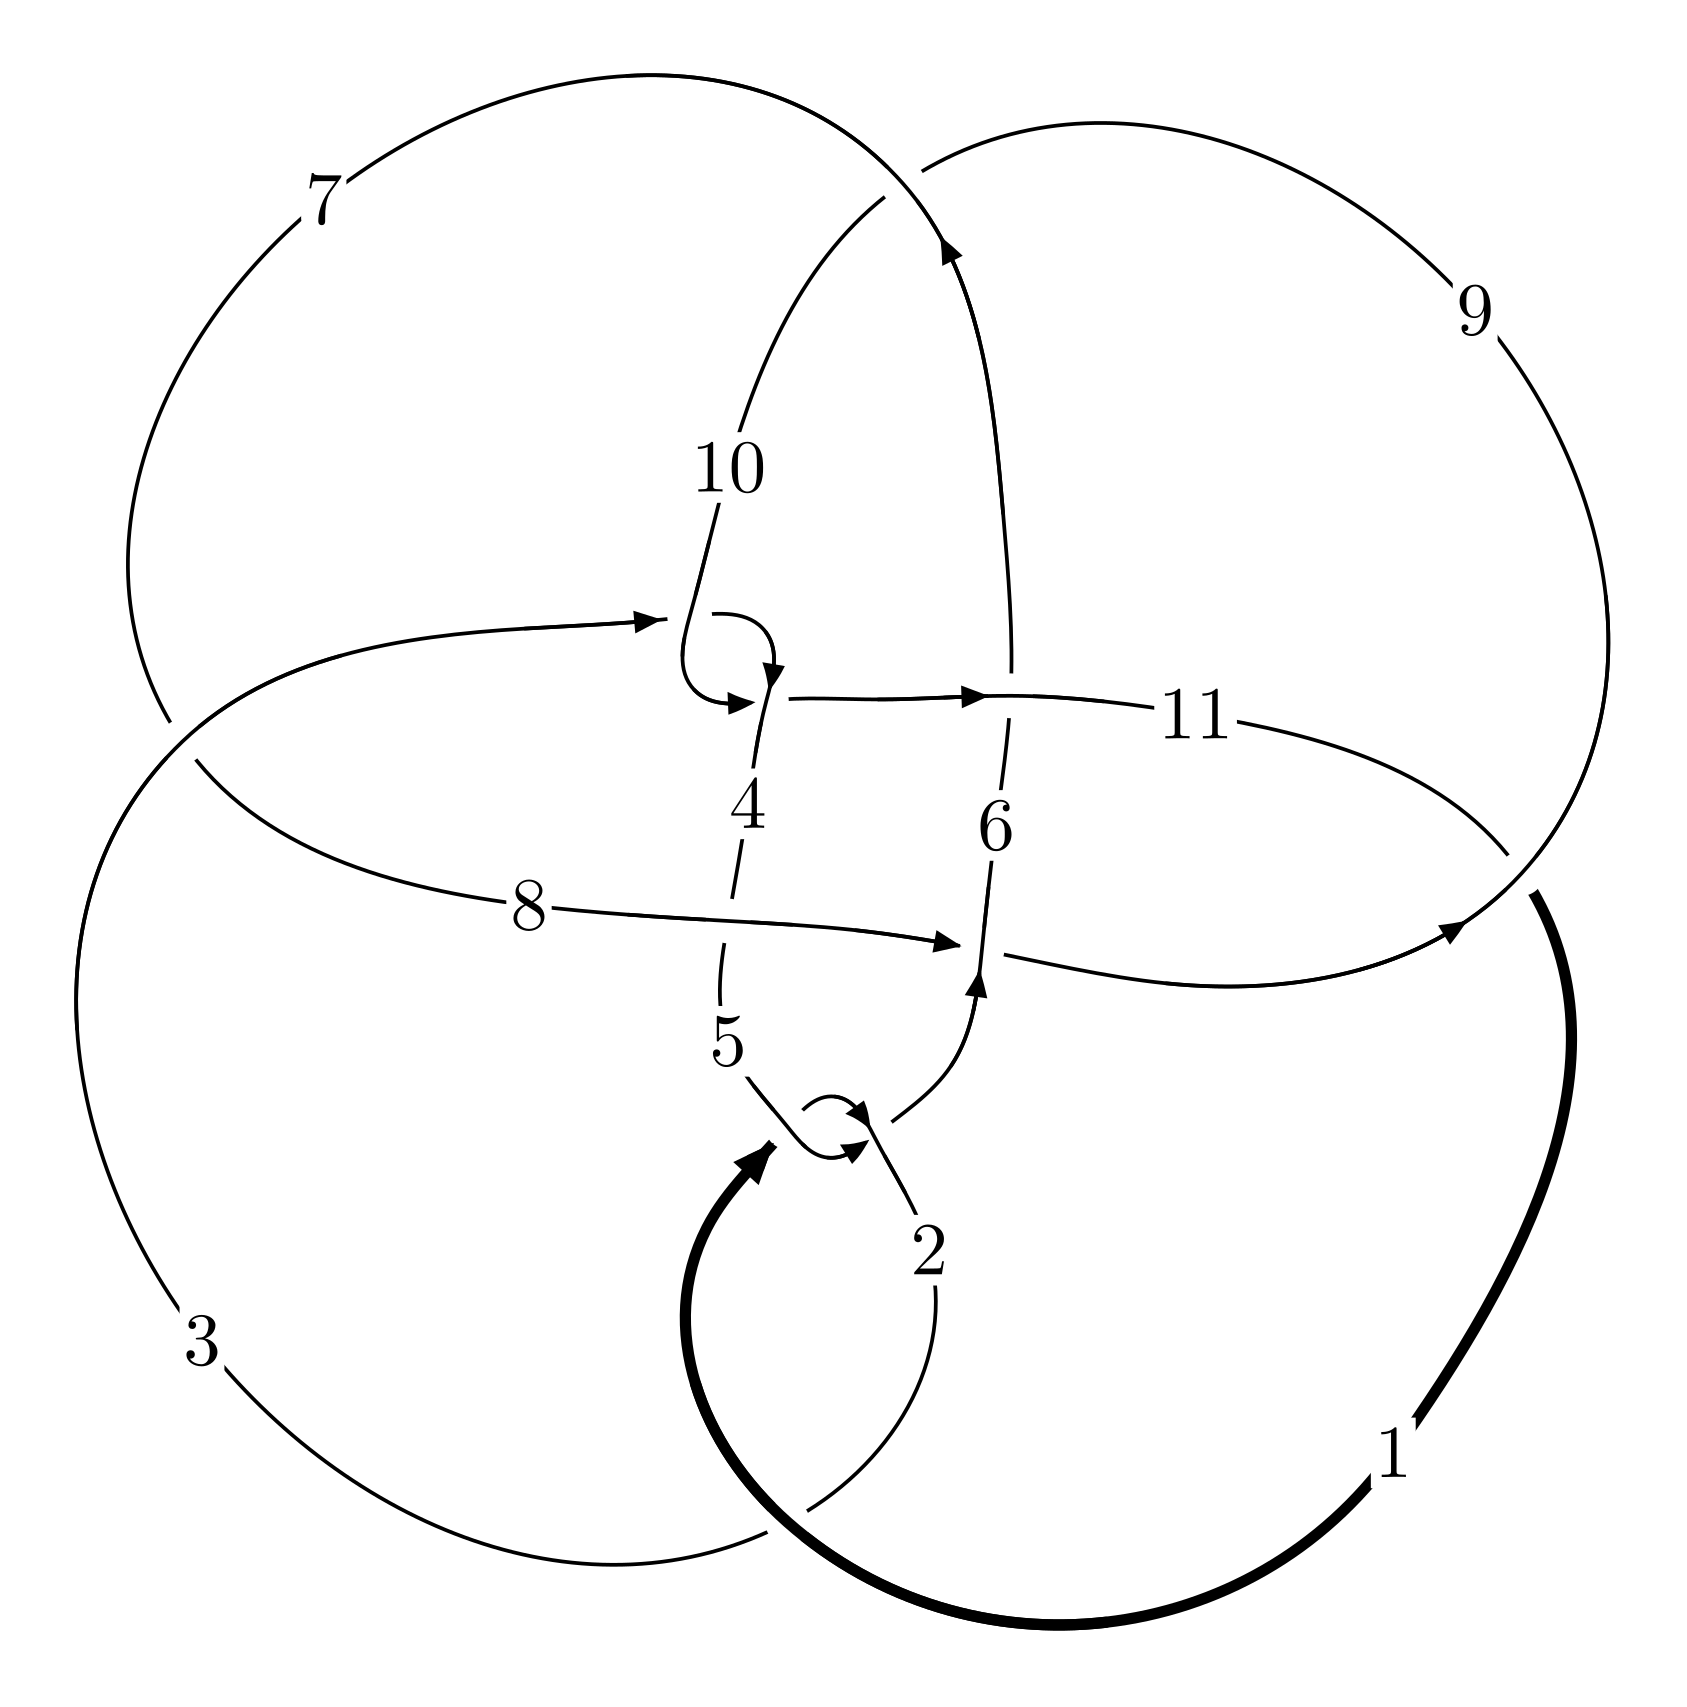
\includegraphics[width=112pt]{../../../GIT/diagram.site/Diagrams/png/374_11a_125.png}\\
\ \ \ A knot diagram\footnotemark}&
\allowdisplaybreaks
\textbf{Linearized knot diagam} \\
\cline{2-2}
 &
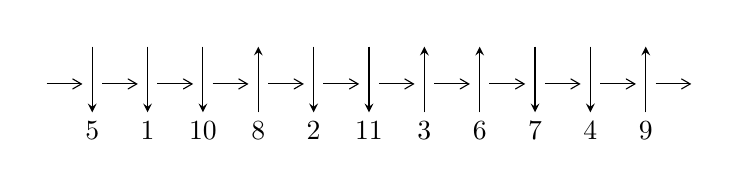
\begin{tikzpicture}[x=20pt, y=17pt]
	% nodes
	\node (C0) at (0, 0) {};
	\node (C1) at (1, 0) {};
	\node (C1U) at (1, +1) {};
	\node (C1D) at (1, -1) {5};

	\node (C2) at (2, 0) {};
	\node (C2U) at (2, +1) {};
	\node (C2D) at (2, -1) {1};

	\node (C3) at (3, 0) {};
	\node (C3U) at (3, +1) {};
	\node (C3D) at (3, -1) {10};

	\node (C4) at (4, 0) {};
	\node (C4U) at (4, +1) {};
	\node (C4D) at (4, -1) {8};

	\node (C5) at (5, 0) {};
	\node (C5U) at (5, +1) {};
	\node (C5D) at (5, -1) {2};

	\node (C6) at (6, 0) {};
	\node (C6U) at (6, +1) {};
	\node (C6D) at (6, -1) {11};

	\node (C7) at (7, 0) {};
	\node (C7U) at (7, +1) {};
	\node (C7D) at (7, -1) {3};

	\node (C8) at (8, 0) {};
	\node (C8U) at (8, +1) {};
	\node (C8D) at (8, -1) {6};

	\node (C9) at (9, 0) {};
	\node (C9U) at (9, +1) {};
	\node (C9D) at (9, -1) {7};

	\node (C10) at (10, 0) {};
	\node (C10U) at (10, +1) {};
	\node (C10D) at (10, -1) {4};

	\node (C11) at (11, 0) {};
	\node (C11U) at (11, +1) {};
	\node (C11D) at (11, -1) {9};
	\node (C12) at (12, 0) {};

	% arrows
	\draw[->,>={angle 60}]
	(C0) edge (C1) (C1) edge (C2) (C2) edge (C3) (C3) edge (C4) (C4) edge (C5) (C5) edge (C6) (C6) edge (C7) (C7) edge (C8) (C8) edge (C9) (C9) edge (C10) (C10) edge (C11) (C11) edge (C12) ;	\draw[->,>=stealth]
	(C1U) edge (C1D) (C2U) edge (C2D) (C3U) edge (C3D) (C4D) edge (C4U) (C5U) edge (C5D) (C6U) edge (C6D) (C7D) edge (C7U) (C8D) edge (C8U) (C9U) edge (C9D) (C10U) edge (C10D) (C11D) edge (C11U) ;
	\end{tikzpicture} \\
\hhline{~~} \\& 
\textbf{Solving Sequence} \\ \cline{2-2} 
 &
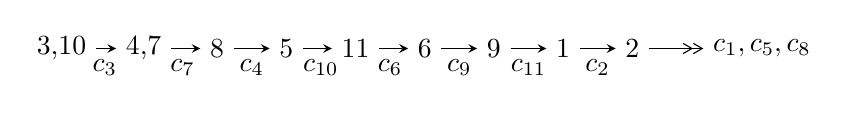
\begin{tikzpicture}[x=25pt, y=7pt]
	% node
	\node (A0) at (-1/8, 0) {3,10};
	\node (A1) at (17/16, 0) {4,7};
	\node (A2) at (17/8, 0) {8};
	\node (A3) at (25/8, 0) {5};
	\node (A4) at (33/8, 0) {11};
	\node (A5) at (41/8, 0) {6};
	\node (A6) at (49/8, 0) {9};
	\node (A7) at (57/8, 0) {1};
	\node (A8) at (65/8, 0) {2};
	\node (C1) at (1/2, -1) {$c_{3}$};
	\node (C2) at (13/8, -1) {$c_{7}$};
	\node (C3) at (21/8, -1) {$c_{4}$};
	\node (C4) at (29/8, -1) {$c_{10}$};
	\node (C5) at (37/8, -1) {$c_{6}$};
	\node (C6) at (45/8, -1) {$c_{9}$};
	\node (C7) at (53/8, -1) {$c_{11}$};
	\node (C8) at (61/8, -1) {$c_{2}$};
	\node (A9) at (10, 0) {$c_{1},c_{5},c_{8}$};

	% edge
	\draw[->,>=stealth]	
	(A0) edge (A1) (A1) edge (A2) (A2) edge (A3) (A3) edge (A4) (A4) edge (A5) (A5) edge (A6) (A6) edge (A7) (A7) edge (A8) ;
	\draw[->>,>={angle 60}]	
	(A8) edge (A9);
\end{tikzpicture} \\ 

\end{tabular} \\

\footnotetext{
The image of knot diagram is generated by the software ``\textbf{Draw programme}" developed by Andrew Bartholomew(\url{http://www.layer8.co.uk/maths/draw/index.htm\#Running-draw}), where we modified some parts for our purpose(\url{https://github.com/CATsTAILs/LinksPainter}).
}\phantom \\ \newline 
\centering \textbf{Ideals for irreducible components\footnotemark of $X_{\text{par}}$} 
 
\begin{align*}
I^u_{1}&=\langle 
1.84217\times10^{296} u^{107}-5.87629\times10^{295} u^{106}+\cdots+2.24754\times10^{296} b-2.30103\times10^{297},\\
\phantom{I^u_{1}}&\phantom{= \langle  }6.03695\times10^{298} u^{107}+3.59147\times10^{297} u^{106}+\cdots+1.32605\times10^{298} a-3.33008\times10^{300},\\
\phantom{I^u_{1}}&\phantom{= \langle  }u^{108}+u^{107}+\cdots-83 u-59\rangle \\
I^u_{2}&=\langle 
u^{20}-5 u^{18}+\cdots- u^2+b,\;46965 u^{20}+32047 u^{19}+\cdots+721 a+56452,\;u^{21}-6 u^{19}+\cdots+u-1\rangle \\
\\
\end{align*}
\raggedright * 2 irreducible components of $\dim_{\mathbb{C}}=0$, with total 129 representations.\\
\footnotetext{All coefficients of polynomials are rational numbers. But the coefficients are sometimes approximated in decimal forms when there is not enough margin.}
\newpage
\renewcommand{\arraystretch}{1}
\centering \section*{I. $I^u_{1}= \langle 1.84\times10^{296} u^{107}-5.88\times10^{295} u^{106}+\cdots+2.25\times10^{296} b-2.30\times10^{297},\;6.04\times10^{298} u^{107}+3.59\times10^{297} u^{106}+\cdots+1.33\times10^{298} a-3.33\times10^{300},\;u^{108}+u^{107}+\cdots-83 u-59 \rangle$}
\flushleft \textbf{(i) Arc colorings}\\
\begin{tabular}{m{7pt} m{180pt} m{7pt} m{180pt} }
\flushright $a_{3}=$&$\begin{pmatrix}1\\0\end{pmatrix}$ \\
\flushright $a_{10}=$&$\begin{pmatrix}0\\u\end{pmatrix}$ \\
\flushright $a_{4}=$&$\begin{pmatrix}1\\u^2\end{pmatrix}$ \\
\flushright $a_{7}=$&$\begin{pmatrix}-4.55258 u^{107}-0.270839 u^{106}+\cdots+163.283 u+251.128\\-0.819637 u^{107}+0.261454 u^{106}+\cdots+30.2031 u+10.2380\end{pmatrix}$ \\
\flushright $a_{8}=$&$\begin{pmatrix}-5.37222 u^{107}-0.00938531 u^{106}+\cdots+193.486 u+261.366\\-0.819637 u^{107}+0.261454 u^{106}+\cdots+30.2031 u+10.2380\end{pmatrix}$ \\
\flushright $a_{5}=$&$\begin{pmatrix}-6.62397 u^{107}-0.205128 u^{106}+\cdots+183.752 u+334.707\\-2.17222 u^{107}-0.986012 u^{106}+\cdots-26.5179 u+197.181\end{pmatrix}$ \\
\flushright $a_{11}=$&$\begin{pmatrix}- u\\- u^3+u\end{pmatrix}$ \\
\flushright $a_{6}=$&$\begin{pmatrix}-7.55781 u^{107}-0.253371 u^{106}+\cdots+270.915 u+397.061\\-0.697834 u^{107}-0.250517 u^{106}+\cdots-3.85380 u+42.6441\end{pmatrix}$ \\
\flushright $a_{9}=$&$\begin{pmatrix}3.16584 u^{107}-1.50394 u^{106}+\cdots-237.293 u-92.9237\\0.781089 u^{107}-0.0600302 u^{106}+\cdots+9.43331 u-62.4900\end{pmatrix}$ \\
\flushright $a_{1}=$&$\begin{pmatrix}7.79988 u^{107}+1.89245 u^{106}+\cdots-175.618 u-567.148\\-1.58619 u^{107}+0.235617 u^{106}+\cdots+70.8587 u+86.7375\end{pmatrix}$ \\
\flushright $a_{2}=$&$\begin{pmatrix}10.8546 u^{107}+1.12089 u^{106}+\cdots-350.252 u-602.137\\2.49334 u^{107}+1.40596 u^{106}+\cdots+40.6084 u-227.462\end{pmatrix}$\\ \flushright $a_{2}=$&$\begin{pmatrix}10.8546 u^{107}+1.12089 u^{106}+\cdots-350.252 u-602.137\\2.49334 u^{107}+1.40596 u^{106}+\cdots+40.6084 u-227.462\end{pmatrix}$\\&\end{tabular}
\flushleft \textbf{(ii) Obstruction class $= -1$}\\~\\
\flushleft \textbf{(iii) Cusp Shapes $= 0.190628 u^{107}+5.28530 u^{106}+\cdots+317.291 u-531.973$}\\~\\
\newpage\renewcommand{\arraystretch}{1}
\flushleft \textbf{(iv) u-Polynomials at the component}\newline \\
\begin{tabular}{m{50pt}|m{274pt}}
Crossings & \hspace{64pt}u-Polynomials at each crossing \\
\hline $$\begin{aligned}c_{1},c_{5}\end{aligned}$$&$\begin{aligned}
&u^{108}+3 u^{107}+\cdots-10 u-1
\end{aligned}$\\
\hline $$\begin{aligned}c_{2}\end{aligned}$$&$\begin{aligned}
&u^{108}+49 u^{107}+\cdots-24 u+1
\end{aligned}$\\
\hline $$\begin{aligned}c_{3},c_{10}\end{aligned}$$&$\begin{aligned}
&u^{108}+u^{107}+\cdots-83 u-59
\end{aligned}$\\
\hline $$\begin{aligned}c_{4}\end{aligned}$$&$\begin{aligned}
&u^{108}+u^{107}+\cdots+9996 u+1033
\end{aligned}$\\
\hline $$\begin{aligned}c_{6}\end{aligned}$$&$\begin{aligned}
&u^{108}+5 u^{107}+\cdots-40 u+1
\end{aligned}$\\
\hline $$\begin{aligned}c_{7}\end{aligned}$$&$\begin{aligned}
&u^{108}+u^{107}+\cdots-47121 u-5231
\end{aligned}$\\
\hline $$\begin{aligned}c_{8}\end{aligned}$$&$\begin{aligned}
&u^{108}-3 u^{107}+\cdots-554 u-1
\end{aligned}$\\
\hline $$\begin{aligned}c_{9}\end{aligned}$$&$\begin{aligned}
&u^{108}+6 u^{107}+\cdots+4092 u+176
\end{aligned}$\\
\hline $$\begin{aligned}c_{11}\end{aligned}$$&$\begin{aligned}
&u^{108}+11 u^{107}+\cdots+776 u+56
\end{aligned}$\\
\hline
\end{tabular}\\~\\
\newpage\renewcommand{\arraystretch}{1}
\flushleft \textbf{(v) Riley Polynomials at the component}\newline \\
\begin{tabular}{m{50pt}|m{274pt}}
Crossings & \hspace{64pt}Riley Polynomials at each crossing \\
\hline $$\begin{aligned}c_{1},c_{5}\end{aligned}$$&$\begin{aligned}
&y^{108}-49 y^{107}+\cdots+24 y+1
\end{aligned}$\\
\hline $$\begin{aligned}c_{2}\end{aligned}$$&$\begin{aligned}
&y^{108}+27 y^{107}+\cdots+756 y+1
\end{aligned}$\\
\hline $$\begin{aligned}c_{3},c_{10}\end{aligned}$$&$\begin{aligned}
&y^{108}-65 y^{107}+\cdots-78869 y+3481
\end{aligned}$\\
\hline $$\begin{aligned}c_{4}\end{aligned}$$&$\begin{aligned}
&y^{108}-5 y^{107}+\cdots+107533242 y+1067089
\end{aligned}$\\
\hline $$\begin{aligned}c_{6}\end{aligned}$$&$\begin{aligned}
&y^{108}-9 y^{107}+\cdots-94 y+1
\end{aligned}$\\
\hline $$\begin{aligned}c_{7}\end{aligned}$$&$\begin{aligned}
&y^{108}+19 y^{107}+\cdots+1542196425 y+27363361
\end{aligned}$\\
\hline $$\begin{aligned}c_{8}\end{aligned}$$&$\begin{aligned}
&y^{108}-13 y^{107}+\cdots-315250 y+1
\end{aligned}$\\
\hline $$\begin{aligned}c_{9}\end{aligned}$$&$\begin{aligned}
&y^{108}-22 y^{107}+\cdots-5774384 y+30976
\end{aligned}$\\
\hline $$\begin{aligned}c_{11}\end{aligned}$$&$\begin{aligned}
&y^{108}-3 y^{107}+\cdots+93344 y+3136
\end{aligned}$\\
\hline
\end{tabular}\\~\\
\newpage\flushleft \textbf{(vi) Complex Volumes and Cusp Shapes}
$$\begin{array}{c|c|c}  
\text{Solutions to }I^u_{1}& \I (\text{vol} + \sqrt{-1}CS) & \text{Cusp shape}\\
 \hline 
\begin{aligned}
u &= -0.974152 + 0.261389 I \\
a &= -0.03692 + 2.17388 I \\
b &= \phantom{-}0.669974 + 0.537090 I\end{aligned}
 & -0.02612 + 8.87697 I & \phantom{-0.000000 } 0 \\ \hline\begin{aligned}
u &= -0.974152 - 0.261389 I \\
a &= -0.03692 - 2.17388 I \\
b &= \phantom{-}0.669974 - 0.537090 I\end{aligned}
 & -0.02612 - 8.87697 I & \phantom{-0.000000 } 0 \\ \hline\begin{aligned}
u &= \phantom{-}0.947317 + 0.290364 I \\
a &= -0.05100 + 1.88670 I \\
b &= -0.525756 + 0.430022 I\end{aligned}
 & \phantom{-}1.77660 - 4.02492 I & \phantom{-0.000000 } 0 \\ \hline\begin{aligned}
u &= \phantom{-}0.947317 - 0.290364 I \\
a &= -0.05100 - 1.88670 I \\
b &= -0.525756 - 0.430022 I\end{aligned}
 & \phantom{-}1.77660 + 4.02492 I & \phantom{-0.000000 } 0 \\ \hline\begin{aligned}
u &= -0.821343 + 0.549763 I \\
a &= -0.183712 - 0.013594 I \\
b &= -0.810583 + 0.713014 I\end{aligned}
 & -0.01641 + 4.09614 I & \phantom{-0.000000 } 0 \\ \hline\begin{aligned}
u &= -0.821343 - 0.549763 I \\
a &= -0.183712 + 0.013594 I \\
b &= -0.810583 - 0.713014 I\end{aligned}
 & -0.01641 - 4.09614 I & \phantom{-0.000000 } 0 \\ \hline\begin{aligned}
u &= \phantom{-}0.984228 + 0.010410 I \\
a &= \phantom{-}1.18874 + 0.90018 I \\
b &= -0.322699 + 1.182530 I\end{aligned}
 & -4.12669 - 3.67423 I & \phantom{-0.000000 } 0 \\ \hline\begin{aligned}
u &= \phantom{-}0.984228 - 0.010410 I \\
a &= \phantom{-}1.18874 - 0.90018 I \\
b &= -0.322699 - 1.182530 I\end{aligned}
 & -4.12669 + 3.67423 I & \phantom{-0.000000 } 0 \\ \hline\begin{aligned}
u &= -0.962477 + 0.079682 I \\
a &= -0.757415 - 0.539055 I \\
b &= \phantom{-}0.58214 - 1.44592 I\end{aligned}
 & -1.112250 + 0.388404 I & \phantom{-0.000000 } 0 \\ \hline\begin{aligned}
u &= -0.962477 - 0.079682 I \\
a &= -0.757415 + 0.539055 I \\
b &= \phantom{-}0.58214 + 1.44592 I\end{aligned}
 & -1.112250 - 0.388404 I & \phantom{-0.000000 } 0\\
 \hline 
 \end{array}$$\newpage$$\begin{array}{c|c|c}  
\text{Solutions to }I^u_{1}& \I (\text{vol} + \sqrt{-1}CS) & \text{Cusp shape}\\
 \hline 
\begin{aligned}
u &= \phantom{-}0.870704 + 0.410766 I \\
a &= -0.279670 + 1.209090 I \\
b &= -0.103162 + 0.129699 I\end{aligned}
 & \phantom{-}1.64684 - 2.43797 I & \phantom{-0.000000 } 0 \\ \hline\begin{aligned}
u &= \phantom{-}0.870704 - 0.410766 I \\
a &= -0.279670 - 1.209090 I \\
b &= -0.103162 - 0.129699 I\end{aligned}
 & \phantom{-}1.64684 + 2.43797 I & \phantom{-0.000000 } 0 \\ \hline\begin{aligned}
u &= \phantom{-}0.726983 + 0.627227 I \\
a &= \phantom{-}0.509551 - 0.049885 I \\
b &= \phantom{-}0.596579 + 1.069470 I\end{aligned}
 & -0.029889 - 0.257369 I & \phantom{-0.000000 } 0 \\ \hline\begin{aligned}
u &= \phantom{-}0.726983 - 0.627227 I \\
a &= \phantom{-}0.509551 + 0.049885 I \\
b &= \phantom{-}0.596579 - 1.069470 I\end{aligned}
 & -0.029889 + 0.257369 I & \phantom{-0.000000 } 0 \\ \hline\begin{aligned}
u &= -0.127716 + 1.038120 I \\
a &= -0.620092 + 0.238590 I \\
b &= \phantom{-}0.737287 + 0.208133 I\end{aligned}
 & \phantom{-}3.55118 + 3.28339 I & \phantom{-0.000000 } 0 \\ \hline\begin{aligned}
u &= -0.127716 - 1.038120 I \\
a &= -0.620092 - 0.238590 I \\
b &= \phantom{-}0.737287 - 0.208133 I\end{aligned}
 & \phantom{-}3.55118 - 3.28339 I & \phantom{-0.000000 } 0 \\ \hline\begin{aligned}
u &= \phantom{-}0.904734 + 0.285757 I \\
a &= \phantom{-}0.636986 + 0.528069 I \\
b &= -2.20932 - 0.22643 I\end{aligned}
 & \phantom{-}0.67232 - 8.72797 I & \phantom{-0.000000 } 0 \\ \hline\begin{aligned}
u &= \phantom{-}0.904734 - 0.285757 I \\
a &= \phantom{-}0.636986 - 0.528069 I \\
b &= -2.20932 + 0.22643 I\end{aligned}
 & \phantom{-}0.67232 + 8.72797 I & \phantom{-0.000000 } 0 \\ \hline\begin{aligned}
u &= -0.910645 + 0.192506 I \\
a &= -0.58789 + 1.78120 I \\
b &= \phantom{-}0.385944 + 0.804425 I\end{aligned}
 & -2.35042 + 2.26476 I & \phantom{-0.000000 } 0 \\ \hline\begin{aligned}
u &= -0.910645 - 0.192506 I \\
a &= -0.58789 - 1.78120 I \\
b &= \phantom{-}0.385944 - 0.804425 I\end{aligned}
 & -2.35042 - 2.26476 I & \phantom{-0.000000 } 0\\
 \hline 
 \end{array}$$\newpage$$\begin{array}{c|c|c}  
\text{Solutions to }I^u_{1}& \I (\text{vol} + \sqrt{-1}CS) & \text{Cusp shape}\\
 \hline 
\begin{aligned}
u &= -0.903214 + 0.219783 I \\
a &= -0.543275 + 0.336286 I \\
b &= \phantom{-}2.17612 - 0.58688 I\end{aligned}
 & \phantom{-}1.86423 + 3.20245 I & \phantom{-0.000000 } 0 \\ \hline\begin{aligned}
u &= -0.903214 - 0.219783 I \\
a &= -0.543275 - 0.336286 I \\
b &= \phantom{-}2.17612 + 0.58688 I\end{aligned}
 & \phantom{-}1.86423 - 3.20245 I & \phantom{-0.000000 } 0 \\ \hline\begin{aligned}
u &= \phantom{-}1.066670 + 0.106723 I \\
a &= \phantom{-}1.187770 - 0.127686 I \\
b &= -0.630782 - 0.730192 I\end{aligned}
 & -4.84250 - 3.77355 I & \phantom{-0.000000 } 0 \\ \hline\begin{aligned}
u &= \phantom{-}1.066670 - 0.106723 I \\
a &= \phantom{-}1.187770 + 0.127686 I \\
b &= -0.630782 + 0.730192 I\end{aligned}
 & -4.84250 + 3.77355 I & \phantom{-0.000000 } 0 \\ \hline\begin{aligned}
u &= -0.895542 + 0.603288 I \\
a &= \phantom{-}0.630755 + 0.940432 I \\
b &= -0.061847 - 0.334834 I\end{aligned}
 & -0.85408 - 1.78433 I & \phantom{-0.000000 } 0 \\ \hline\begin{aligned}
u &= -0.895542 - 0.603288 I \\
a &= \phantom{-}0.630755 - 0.940432 I \\
b &= -0.061847 + 0.334834 I\end{aligned}
 & -0.85408 + 1.78433 I & \phantom{-0.000000 } 0 \\ \hline\begin{aligned}
u &= \phantom{-}0.534951 + 0.717555 I \\
a &= \phantom{-}0.906959 - 0.057499 I \\
b &= -0.006657 + 1.274660 I\end{aligned}
 & \phantom{-}0.45026 - 4.79181 I & \phantom{-0.000000 } 0 \\ \hline\begin{aligned}
u &= \phantom{-}0.534951 - 0.717555 I \\
a &= \phantom{-}0.906959 + 0.057499 I \\
b &= -0.006657 - 1.274660 I\end{aligned}
 & \phantom{-}0.45026 + 4.79181 I & \phantom{-0.000000 } 0 \\ \hline\begin{aligned}
u &= \phantom{-}0.978238 + 0.528279 I \\
a &= \phantom{-}0.830922 - 0.731888 I \\
b &= \phantom{-}0.130929 + 1.208130 I\end{aligned}
 & -4.29595 + 1.62915 I & \phantom{-0.000000 } 0 \\ \hline\begin{aligned}
u &= \phantom{-}0.978238 - 0.528279 I \\
a &= \phantom{-}0.830922 + 0.731888 I \\
b &= \phantom{-}0.130929 - 1.208130 I\end{aligned}
 & -4.29595 - 1.62915 I & \phantom{-0.000000 } 0\\
 \hline 
 \end{array}$$\newpage$$\begin{array}{c|c|c}  
\text{Solutions to }I^u_{1}& \I (\text{vol} + \sqrt{-1}CS) & \text{Cusp shape}\\
 \hline 
\begin{aligned}
u &= \phantom{-}0.132879 + 1.112260 I \\
a &= \phantom{-}0.490463 + 0.469192 I \\
b &= -0.676211 - 0.179571 I\end{aligned}
 & \phantom{-}4.46641 + 2.42852 I & \phantom{-0.000000 } 0 \\ \hline\begin{aligned}
u &= \phantom{-}0.132879 - 1.112260 I \\
a &= \phantom{-}0.490463 - 0.469192 I \\
b &= -0.676211 + 0.179571 I\end{aligned}
 & \phantom{-}4.46641 - 2.42852 I & \phantom{-0.000000 } 0 \\ \hline\begin{aligned}
u &= -0.163742 + 1.117370 I \\
a &= -0.541417 + 0.966843 I \\
b &= \phantom{-}0.807554 - 1.027800 I\end{aligned}
 & \phantom{-}0.81340 - 12.59150 I & \phantom{-0.000000 } 0 \\ \hline\begin{aligned}
u &= -0.163742 - 1.117370 I \\
a &= -0.541417 - 0.966843 I \\
b &= \phantom{-}0.807554 + 1.027800 I\end{aligned}
 & \phantom{-}0.81340 + 12.59150 I & \phantom{-0.000000 } 0 \\ \hline\begin{aligned}
u &= \phantom{-}0.169000 + 1.121780 I \\
a &= \phantom{-}0.518616 + 0.885953 I \\
b &= -0.779199 - 0.872057 I\end{aligned}
 & \phantom{-}2.97894 + 6.84382 I & \phantom{-0.000000 } 0 \\ \hline\begin{aligned}
u &= \phantom{-}0.169000 - 1.121780 I \\
a &= \phantom{-}0.518616 - 0.885953 I \\
b &= -0.779199 + 0.872057 I\end{aligned}
 & \phantom{-}2.97894 - 6.84382 I & \phantom{-0.000000 } 0 \\ \hline\begin{aligned}
u &= -0.197636 + 1.125790 I \\
a &= -0.304167 + 0.875966 I \\
b &= \phantom{-}0.421882 - 0.817706 I\end{aligned}
 & -3.21665 - 3.93627 I & \phantom{-0.000000 } 0 \\ \hline\begin{aligned}
u &= -0.197636 - 1.125790 I \\
a &= -0.304167 - 0.875966 I \\
b &= \phantom{-}0.421882 + 0.817706 I\end{aligned}
 & -3.21665 + 3.93627 I & \phantom{-0.000000 } 0 \\ \hline\begin{aligned}
u &= -0.834451\phantom{ +0.000000I} \\
a &= \phantom{-}0.489255\phantom{ +0.000000I} \\
b &= -0.665164\phantom{ +0.000000I}\end{aligned}
 & -1.38852\phantom{ +0.000000I} & \phantom{-0.000000 } 0 \\ \hline\begin{aligned}
u &= -0.398165 + 0.716767 I \\
a &= -1.019530 - 0.052785 I \\
b &= \phantom{-}0.269627 + 1.067180 I\end{aligned}
 & \phantom{-}1.014240 + 0.642379 I & \phantom{-0.000000 } 0\\
 \hline 
 \end{array}$$\newpage$$\begin{array}{c|c|c}  
\text{Solutions to }I^u_{1}& \I (\text{vol} + \sqrt{-1}CS) & \text{Cusp shape}\\
 \hline 
\begin{aligned}
u &= -0.398165 - 0.716767 I \\
a &= -1.019530 + 0.052785 I \\
b &= \phantom{-}0.269627 - 1.067180 I\end{aligned}
 & \phantom{-}1.014240 - 0.642379 I & \phantom{-0.000000 } 0 \\ \hline\begin{aligned}
u &= \phantom{-}1.120110 + 0.400495 I \\
a &= \phantom{-}1.256760 + 0.503964 I \\
b &= -1.32125 + 1.02155 I\end{aligned}
 & -3.30658 - 4.72348 I & \phantom{-0.000000 } 0 \\ \hline\begin{aligned}
u &= \phantom{-}1.120110 - 0.400495 I \\
a &= \phantom{-}1.256760 - 0.503964 I \\
b &= -1.32125 - 1.02155 I\end{aligned}
 & -3.30658 + 4.72348 I & \phantom{-0.000000 } 0 \\ \hline\begin{aligned}
u &= -1.133440 + 0.447556 I \\
a &= -1.40826 + 0.51127 I \\
b &= \phantom{-}1.33693 + 1.47390 I\end{aligned}
 & -4.55602 + 8.69100 I & \phantom{-0.000000 } 0 \\ \hline\begin{aligned}
u &= -1.133440 - 0.447556 I \\
a &= -1.40826 - 0.51127 I \\
b &= \phantom{-}1.33693 - 1.47390 I\end{aligned}
 & -4.55602 - 8.69100 I & \phantom{-0.000000 } 0 \\ \hline\begin{aligned}
u &= -0.735283 + 0.258478 I \\
a &= \phantom{-}0.131993 - 1.382150 I \\
b &= -0.91333 - 1.27864 I\end{aligned}
 & \phantom{-}2.25905 - 0.80230 I & \phantom{-0.000000 } 0 \\ \hline\begin{aligned}
u &= -0.735283 - 0.258478 I \\
a &= \phantom{-}0.131993 + 1.382150 I \\
b &= -0.91333 + 1.27864 I\end{aligned}
 & \phantom{-}2.25905 + 0.80230 I & \phantom{-0.000000 } 0 \\ \hline\begin{aligned}
u &= \phantom{-}1.136570 + 0.494217 I \\
a &= \phantom{-}1.232080 - 0.166947 I \\
b &= -0.27028 + 1.43055 I\end{aligned}
 & -5.27860 - 5.21926 I & \phantom{-0.000000 } 0 \\ \hline\begin{aligned}
u &= \phantom{-}1.136570 - 0.494217 I \\
a &= \phantom{-}1.232080 + 0.166947 I \\
b &= -0.27028 - 1.43055 I\end{aligned}
 & -5.27860 + 5.21926 I & \phantom{-0.000000 } 0 \\ \hline\begin{aligned}
u &= \phantom{-}1.194790 + 0.353430 I \\
a &= \phantom{-}1.217590 + 0.419263 I \\
b &= -0.797116 + 0.838560 I\end{aligned}
 & -3.57518 - 4.92310 I & \phantom{-0.000000 } 0\\
 \hline 
 \end{array}$$\newpage$$\begin{array}{c|c|c}  
\text{Solutions to }I^u_{1}& \I (\text{vol} + \sqrt{-1}CS) & \text{Cusp shape}\\
 \hline 
\begin{aligned}
u &= \phantom{-}1.194790 - 0.353430 I \\
a &= \phantom{-}1.217590 - 0.419263 I \\
b &= -0.797116 - 0.838560 I\end{aligned}
 & -3.57518 + 4.92310 I & \phantom{-0.000000 } 0 \\ \hline\begin{aligned}
u &= -1.073590 + 0.645480 I \\
a &= -0.696546 - 0.301950 I \\
b &= \phantom{-}0.115944 + 1.063470 I\end{aligned}
 & -1.85031 + 2.56322 I & \phantom{-0.000000 } 0 \\ \hline\begin{aligned}
u &= -1.073590 - 0.645480 I \\
a &= -0.696546 + 0.301950 I \\
b &= \phantom{-}0.115944 - 1.063470 I\end{aligned}
 & -1.85031 - 2.56322 I & \phantom{-0.000000 } 0 \\ \hline\begin{aligned}
u &= -1.167860 + 0.453399 I \\
a &= -1.44149 + 0.26526 I \\
b &= \phantom{-}0.80245 + 1.59814 I\end{aligned}
 & -5.45176 + 2.92622 I & \phantom{-0.000000 } 0 \\ \hline\begin{aligned}
u &= -1.167860 - 0.453399 I \\
a &= -1.44149 - 0.26526 I \\
b &= \phantom{-}0.80245 - 1.59814 I\end{aligned}
 & -5.45176 - 2.92622 I & \phantom{-0.000000 } 0 \\ \hline\begin{aligned}
u &= -1.240790 + 0.240630 I \\
a &= \phantom{-}0.534776 - 0.182654 I \\
b &= -1.31764 - 1.44251 I\end{aligned}
 & -1.79007 + 3.25272 I & \phantom{-0.000000 } 0 \\ \hline\begin{aligned}
u &= -1.240790 - 0.240630 I \\
a &= \phantom{-}0.534776 + 0.182654 I \\
b &= -1.31764 + 1.44251 I\end{aligned}
 & -1.79007 - 3.25272 I & \phantom{-0.000000 } 0 \\ \hline\begin{aligned}
u &= \phantom{-}0.650808 + 0.342791 I \\
a &= -0.34559 - 1.62139 I \\
b &= \phantom{-}1.19891 - 0.98678 I\end{aligned}
 & \phantom{-}1.33081 + 5.80685 I & \phantom{-0.000000 } 0. - 2.96583 I \\ \hline\begin{aligned}
u &= \phantom{-}0.650808 - 0.342791 I \\
a &= -0.34559 + 1.62139 I \\
b &= \phantom{-}1.19891 + 0.98678 I\end{aligned}
 & \phantom{-}1.33081 - 5.80685 I & \phantom{-0.000000 -}0. + 2.96583 I \\ \hline\begin{aligned}
u &= -1.246090 + 0.227495 I \\
a &= -1.342510 + 0.414670 I \\
b &= \phantom{-}0.294925 + 0.427196 I\end{aligned}
 & -5.57876 + 2.04823 I & \phantom{-0.000000 } 0\\
 \hline 
 \end{array}$$\newpage$$\begin{array}{c|c|c}  
\text{Solutions to }I^u_{1}& \I (\text{vol} + \sqrt{-1}CS) & \text{Cusp shape}\\
 \hline 
\begin{aligned}
u &= -1.246090 - 0.227495 I \\
a &= -1.342510 - 0.414670 I \\
b &= \phantom{-}0.294925 - 0.427196 I\end{aligned}
 & -5.57876 - 2.04823 I & \phantom{-0.000000 } 0 \\ \hline\begin{aligned}
u &= \phantom{-}1.230250 + 0.309018 I \\
a &= -0.629731 - 0.227256 I \\
b &= \phantom{-}1.05197 - 1.70214 I\end{aligned}
 & -3.85058 - 9.33974 I & \phantom{-0.000000 } 0 \\ \hline\begin{aligned}
u &= \phantom{-}1.230250 - 0.309018 I \\
a &= -0.629731 + 0.227256 I \\
b &= \phantom{-}1.05197 + 1.70214 I\end{aligned}
 & -3.85058 + 9.33974 I & \phantom{-0.000000 } 0 \\ \hline\begin{aligned}
u &= -0.589715 + 0.333188 I \\
a &= \phantom{-}0.771112 - 0.727221 I \\
b &= -0.700623 + 0.496327 I\end{aligned}
 & -1.78626 + 0.19440 I & -6.62499 - 2.10710 I \\ \hline\begin{aligned}
u &= -0.589715 - 0.333188 I \\
a &= \phantom{-}0.771112 + 0.727221 I \\
b &= -0.700623 - 0.496327 I\end{aligned}
 & -1.78626 - 0.19440 I & -6.62499 + 2.10710 I \\ \hline\begin{aligned}
u &= -0.351167 + 0.578931 I \\
a &= \phantom{-}0.78828 + 1.37252 I \\
b &= -0.829992 - 0.595666 I\end{aligned}
 & \phantom{-}0.49504 + 6.34073 I & -1.73992 - 6.59022 I \\ \hline\begin{aligned}
u &= -0.351167 - 0.578931 I \\
a &= \phantom{-}0.78828 - 1.37252 I \\
b &= -0.829992 + 0.595666 I\end{aligned}
 & \phantom{-}0.49504 - 6.34073 I & -1.73992 + 6.59022 I \\ \hline\begin{aligned}
u &= -0.621401 + 0.199241 I \\
a &= \phantom{-}2.07344 - 0.92194 I \\
b &= -1.201380 + 0.401495 I\end{aligned}
 & \phantom{-}1.06241 - 6.45710 I & \phantom{-0.000000 -}0. + 1.42723 I \\ \hline\begin{aligned}
u &= -0.621401 - 0.199241 I \\
a &= \phantom{-}2.07344 + 0.92194 I \\
b &= -1.201380 - 0.401495 I\end{aligned}
 & \phantom{-}1.06241 + 6.45710 I & \phantom{-0.000000 } 0. - 1.42723 I \\ \hline\begin{aligned}
u &= -0.052871 + 0.646559 I \\
a &= \phantom{-}0.41145 - 1.50671 I \\
b &= -0.382161 + 1.102240 I\end{aligned}
 & -2.32226 + 1.24315 I & -7.51601 - 1.77666 I\\
 \hline 
 \end{array}$$\newpage$$\begin{array}{c|c|c}  
\text{Solutions to }I^u_{1}& \I (\text{vol} + \sqrt{-1}CS) & \text{Cusp shape}\\
 \hline 
\begin{aligned}
u &= -0.052871 - 0.646559 I \\
a &= \phantom{-}0.41145 + 1.50671 I \\
b &= -0.382161 - 1.102240 I\end{aligned}
 & -2.32226 - 1.24315 I & -7.51601 + 1.77666 I \\ \hline\begin{aligned}
u &= -1.326700 + 0.305400 I \\
a &= -1.235880 + 0.564675 I \\
b &= \phantom{-}0.259224 + 0.925110 I\end{aligned}
 & -5.13430 + 8.04503 I & \phantom{-0.000000 } 0 \\ \hline\begin{aligned}
u &= -1.326700 - 0.305400 I \\
a &= -1.235880 - 0.564675 I \\
b &= \phantom{-}0.259224 - 0.925110 I\end{aligned}
 & -5.13430 - 8.04503 I & \phantom{-0.000000 } 0 \\ \hline\begin{aligned}
u &= \phantom{-}1.317900 + 0.402678 I \\
a &= \phantom{-}1.078710 + 0.489570 I \\
b &= -0.474582 + 1.090480 I\end{aligned}
 & -3.99132 - 4.54373 I & \phantom{-0.000000 } 0 \\ \hline\begin{aligned}
u &= \phantom{-}1.317900 - 0.402678 I \\
a &= \phantom{-}1.078710 - 0.489570 I \\
b &= -0.474582 - 1.090480 I\end{aligned}
 & -3.99132 + 4.54373 I & \phantom{-0.000000 } 0 \\ \hline\begin{aligned}
u &= -0.179585 + 0.579606 I \\
a &= \phantom{-}0.83381 - 1.86662 I \\
b &= -0.947899 + 0.787439 I\end{aligned}
 & -1.83419 - 4.63645 I & -4.58372 + 7.30891 I \\ \hline\begin{aligned}
u &= -0.179585 - 0.579606 I \\
a &= \phantom{-}0.83381 + 1.86662 I \\
b &= -0.947899 - 0.787439 I\end{aligned}
 & -1.83419 + 4.63645 I & -4.58372 - 7.30891 I \\ \hline\begin{aligned}
u &= \phantom{-}0.568576 + 0.208009 I \\
a &= -2.01454 - 0.40120 I \\
b &= \phantom{-}1.136210 + 0.244875 I\end{aligned}
 & \phantom{-}2.86820 + 1.36185 I & \phantom{-}3.07135 + 2.06335 I \\ \hline\begin{aligned}
u &= \phantom{-}0.568576 - 0.208009 I \\
a &= -2.01454 + 0.40120 I \\
b &= \phantom{-}1.136210 - 0.244875 I\end{aligned}
 & \phantom{-}2.86820 - 1.36185 I & \phantom{-}3.07135 - 2.06335 I \\ \hline\begin{aligned}
u &= \phantom{-}1.368310 + 0.298986 I \\
a &= -0.624843 - 0.019539 I \\
b &= \phantom{-}0.448426 - 1.103470 I\end{aligned}
 & -8.89731 - 0.89969 I & \phantom{-0.000000 } 0\\
 \hline 
 \end{array}$$\newpage$$\begin{array}{c|c|c}  
\text{Solutions to }I^u_{1}& \I (\text{vol} + \sqrt{-1}CS) & \text{Cusp shape}\\
 \hline 
\begin{aligned}
u &= \phantom{-}1.368310 - 0.298986 I \\
a &= -0.624843 + 0.019539 I \\
b &= \phantom{-}0.448426 + 1.103470 I\end{aligned}
 & -8.89731 + 0.89969 I & \phantom{-0.000000 } 0 \\ \hline\begin{aligned}
u &= \phantom{-}0.435771 + 0.408529 I \\
a &= -1.26938 + 1.01935 I \\
b &= \phantom{-}0.914517 - 0.262108 I\end{aligned}
 & \phantom{-}2.65024 - 1.18829 I & \phantom{-}2.48161 + 2.04057 I \\ \hline\begin{aligned}
u &= \phantom{-}0.435771 - 0.408529 I \\
a &= -1.26938 - 1.01935 I \\
b &= \phantom{-}0.914517 + 0.262108 I\end{aligned}
 & \phantom{-}2.65024 + 1.18829 I & \phantom{-}2.48161 - 2.04057 I \\ \hline\begin{aligned}
u &= -1.310200 + 0.507870 I \\
a &= \phantom{-}0.687774 - 0.140558 I \\
b &= -1.022390 - 0.630758 I\end{aligned}
 & -0.17375 + 2.12643 I & \phantom{-0.000000 } 0 \\ \hline\begin{aligned}
u &= -1.310200 - 0.507870 I \\
a &= \phantom{-}0.687774 + 0.140558 I \\
b &= -1.022390 + 0.630758 I\end{aligned}
 & -0.17375 - 2.12643 I & \phantom{-0.000000 } 0 \\ \hline\begin{aligned}
u &= \phantom{-}1.30647 + 0.56763 I \\
a &= -0.847975 - 0.175210 I \\
b &= \phantom{-}1.050390 - 0.899685 I\end{aligned}
 & \phantom{-}0.76601 - 8.29993 I & \phantom{-0.000000 } 0 \\ \hline\begin{aligned}
u &= \phantom{-}1.30647 - 0.56763 I \\
a &= -0.847975 + 0.175210 I \\
b &= \phantom{-}1.050390 + 0.899685 I\end{aligned}
 & \phantom{-}0.76601 + 8.29993 I & \phantom{-0.000000 } 0 \\ \hline\begin{aligned}
u &= \phantom{-}1.30666 + 0.59592 I \\
a &= -1.114890 - 0.225093 I \\
b &= \phantom{-}1.01748 - 1.35533 I\end{aligned}
 & -0.60805 - 12.89860 I & \phantom{-0.000000 } 0 \\ \hline\begin{aligned}
u &= \phantom{-}1.30666 - 0.59592 I \\
a &= -1.114890 + 0.225093 I \\
b &= \phantom{-}1.01748 + 1.35533 I\end{aligned}
 & -0.60805 + 12.89860 I & \phantom{-0.000000 } 0 \\ \hline\begin{aligned}
u &= -1.30939 + 0.59543 I \\
a &= \phantom{-}1.086590 - 0.077025 I \\
b &= -0.80339 - 1.23187 I\end{aligned}
 & -6.77231 + 10.02240 I & \phantom{-0.000000 } 0\\
 \hline 
 \end{array}$$\newpage$$\begin{array}{c|c|c}  
\text{Solutions to }I^u_{1}& \I (\text{vol} + \sqrt{-1}CS) & \text{Cusp shape}\\
 \hline 
\begin{aligned}
u &= -1.30939 - 0.59543 I \\
a &= \phantom{-}1.086590 + 0.077025 I \\
b &= -0.80339 + 1.23187 I\end{aligned}
 & -6.77231 - 10.02240 I & \phantom{-0.000000 } 0 \\ \hline\begin{aligned}
u &= -1.30900 + 0.59703 I \\
a &= \phantom{-}1.179420 - 0.236168 I \\
b &= -0.99652 - 1.46631 I\end{aligned}
 & -2.7876 + 18.6455 I & \phantom{-0.000000 } 0 \\ \hline\begin{aligned}
u &= -1.30900 - 0.59703 I \\
a &= \phantom{-}1.179420 + 0.236168 I \\
b &= -0.99652 + 1.46631 I\end{aligned}
 & -2.7876 - 18.6455 I & \phantom{-0.000000 } 0 \\ \hline\begin{aligned}
u &= -1.44914 + 0.24366 I \\
a &= \phantom{-}0.550715 + 0.054229 I \\
b &= -0.104588 - 0.667664 I\end{aligned}
 & -2.85677 - 1.64370 I & \phantom{-0.000000 } 0 \\ \hline\begin{aligned}
u &= -1.44914 - 0.24366 I \\
a &= \phantom{-}0.550715 - 0.054229 I \\
b &= -0.104588 + 0.667664 I\end{aligned}
 & -2.85677 + 1.64370 I & \phantom{-0.000000 } 0 \\ \hline\begin{aligned}
u &= -0.027355 + 0.526426 I \\
a &= -1.27042 - 1.03315 I \\
b &= \phantom{-}0.397552 + 0.647777 I\end{aligned}
 & -0.10044 + 1.46604 I & -1.33207 - 4.65115 I \\ \hline\begin{aligned}
u &= -0.027355 - 0.526426 I \\
a &= -1.27042 + 1.03315 I \\
b &= \phantom{-}0.397552 - 0.647777 I\end{aligned}
 & -0.10044 - 1.46604 I & -1.33207 + 4.65115 I \\ \hline\begin{aligned}
u &= \phantom{-}0.296819 + 0.409793 I \\
a &= -0.83453 - 2.24685 I \\
b &= \phantom{-}0.972948 + 0.114369 I\end{aligned}
 & -0.86286 + 1.24545 I & \phantom{-}0.709038 + 0.323843 I \\ \hline\begin{aligned}
u &= \phantom{-}0.296819 - 0.409793 I \\
a &= -0.83453 + 2.24685 I \\
b &= \phantom{-}0.972948 - 0.114369 I\end{aligned}
 & -0.86286 - 1.24545 I & \phantom{-}0.709038 - 0.323843 I \\ \hline\begin{aligned}
u &= -1.35572 + 0.64284 I \\
a &= -0.609435 + 0.254910 I \\
b &= \phantom{-}0.513726 + 0.977254 I\end{aligned}
 & -0.11523 + 4.15027 I & \phantom{-0.000000 } 0\\
 \hline 
 \end{array}$$\newpage$$\begin{array}{c|c|c}  
\text{Solutions to }I^u_{1}& \I (\text{vol} + \sqrt{-1}CS) & \text{Cusp shape}\\
 \hline 
\begin{aligned}
u &= -1.35572 - 0.64284 I \\
a &= -0.609435 - 0.254910 I \\
b &= \phantom{-}0.513726 - 0.977254 I\end{aligned}
 & -0.11523 - 4.15027 I & \phantom{-0.000000 } 0 \\ \hline\begin{aligned}
u &= \phantom{-}1.47738 + 0.29180 I \\
a &= -0.576871 + 0.099376 I \\
b &= -0.086794 - 0.812436 I\end{aligned}
 & -4.87730 + 7.27293 I & \phantom{-0.000000 } 0 \\ \hline\begin{aligned}
u &= \phantom{-}1.47738 - 0.29180 I \\
a &= -0.576871 - 0.099376 I \\
b &= -0.086794 + 0.812436 I\end{aligned}
 & -4.87730 - 7.27293 I & \phantom{-0.000000 } 0 \\ \hline\begin{aligned}
u &= \phantom{-}1.40109 + 0.57788 I \\
a &= \phantom{-}0.653418 + 0.408344 I \\
b &= -0.599849 + 1.050720 I\end{aligned}
 & -1.23164 - 9.21086 I & \phantom{-0.000000 } 0 \\ \hline\begin{aligned}
u &= \phantom{-}1.40109 - 0.57788 I \\
a &= \phantom{-}0.653418 - 0.408344 I \\
b &= -0.599849 - 1.050720 I\end{aligned}
 & -1.23164 + 9.21086 I & \phantom{-0.000000 } 0 \\ \hline\begin{aligned}
u &= -0.21671 + 1.52116 I \\
a &= \phantom{-}0.0068364 - 0.0753318 I \\
b &= -0.013805 + 0.393561 I\end{aligned}
 & \phantom{-}4.02171 + 2.95510 I & \phantom{-0.000000 } 0 \\ \hline\begin{aligned}
u &= -0.21671 - 1.52116 I \\
a &= \phantom{-}0.0068364 + 0.0753318 I \\
b &= -0.013805 - 0.393561 I\end{aligned}
 & \phantom{-}4.02171 - 2.95510 I & \phantom{-0.000000 } 0 \\ \hline\begin{aligned}
u &= \phantom{-}1.68133\phantom{ +0.000000I} \\
a &= -0.497549\phantom{ +0.000000I} \\
b &= \phantom{-}0.905522\phantom{ +0.000000I}\end{aligned}
 & -10.1758\phantom{ +0.000000I} & \phantom{-0.000000 } 0\\
 \hline 
 \end{array}$$\newpage\newpage\renewcommand{\arraystretch}{1}
\centering \section*{II. $I^u_{2}= \langle u^{20}-5 u^{18}+\cdots- u^2+b,\;46965 u^{20}+32047 u^{19}+\cdots+721 a+56452,\;u^{21}-6 u^{19}+\cdots+u-1 \rangle$}
\flushleft \textbf{(i) Arc colorings}\\
\begin{tabular}{m{7pt} m{180pt} m{7pt} m{180pt} }
\flushright $a_{3}=$&$\begin{pmatrix}1\\0\end{pmatrix}$ \\
\flushright $a_{10}=$&$\begin{pmatrix}0\\u\end{pmatrix}$ \\
\flushright $a_{4}=$&$\begin{pmatrix}1\\u^2\end{pmatrix}$ \\
\flushright $a_{7}=$&$\begin{pmatrix}-65.1387 u^{20}-44.4480 u^{19}+\cdots-29.5784 u-78.2968\\- u^{20}+5 u^{18}+\cdots+8 u^3+u^2\end{pmatrix}$ \\
\flushright $a_{8}=$&$\begin{pmatrix}-66.1387 u^{20}-44.4480 u^{19}+\cdots-29.5784 u-78.2968\\- u^{20}+5 u^{18}+\cdots+8 u^3+u^2\end{pmatrix}$ \\
\flushright $a_{5}=$&$\begin{pmatrix}45.5978 u^{20}+35.4008 u^{19}+\cdots+21.6227 u+70.7393\\-46.7642 u^{20}-34.3384 u^{19}+\cdots-21.9168 u-69.2954\end{pmatrix}$ \\
\flushright $a_{11}=$&$\begin{pmatrix}- u\\- u^3+u\end{pmatrix}$ \\
\flushright $a_{6}=$&$\begin{pmatrix}-83.4924 u^{20}-55.9404 u^{19}+\cdots-39.7032 u-99.3537\\7.41331 u^{20}+5.59501 u^{19}+\cdots+3.26352 u+9.56449\end{pmatrix}$ \\
\flushright $a_{9}=$&$\begin{pmatrix}73.8960 u^{20}+47.9140 u^{19}+\cdots+53.3162 u+104.277\\-70.2954 u^{20}-46.7642 u^{19}+\cdots-43.2219 u-91.2122\end{pmatrix}$ \\
\flushright $a_{1}=$&$\begin{pmatrix}-2.38974 u^{20}+0.771151 u^{19}+\cdots-21.2552 u-13.2940\\52.3856 u^{20}+34.1054 u^{19}+\cdots+37.5479 u+71.3051\end{pmatrix}$ \\
\flushright $a_{2}=$&$\begin{pmatrix}-77.2302 u^{20}-53.1637 u^{19}+\cdots-63.1401 u-116.053\\80.0361 u^{20}+55.7365 u^{19}+\cdots+53.1304 u+119.237\end{pmatrix}$\\ \flushright $a_{2}=$&$\begin{pmatrix}-77.2302 u^{20}-53.1637 u^{19}+\cdots-63.1401 u-116.053\\80.0361 u^{20}+55.7365 u^{19}+\cdots+53.1304 u+119.237\end{pmatrix}$\\&\end{tabular}
\flushleft \textbf{(ii) Obstruction class $= 1$}\\~\\
\flushleft \textbf{(iii) Cusp Shapes $= -\frac{221218}{721} u^{20}-\frac{159840}{721} u^{19}+\cdots-\frac{126596}{721} u-\frac{319747}{721}$}\\~\\
\newpage\renewcommand{\arraystretch}{1}
\flushleft \textbf{(iv) u-Polynomials at the component}\newline \\
\begin{tabular}{m{50pt}|m{274pt}}
Crossings & \hspace{64pt}u-Polynomials at each crossing \\
\hline $$\begin{aligned}c_{1}\end{aligned}$$&$\begin{aligned}
&u^{21}+2 u^{20}+\cdots-2 u+1
\end{aligned}$\\
\hline $$\begin{aligned}c_{2}\end{aligned}$$&$\begin{aligned}
&u^{21}+12 u^{20}+\cdots+16 u+1
\end{aligned}$\\
\hline $$\begin{aligned}c_{3}\end{aligned}$$&$\begin{aligned}
&u^{21}-6 u^{19}+\cdots+u-1
\end{aligned}$\\
\hline $$\begin{aligned}c_{4}\end{aligned}$$&$\begin{aligned}
&u^{21}+4 u^{19}+\cdots+4 u-1
\end{aligned}$\\
\hline $$\begin{aligned}c_{5}\end{aligned}$$&$\begin{aligned}
&u^{21}-2 u^{20}+\cdots-2 u-1
\end{aligned}$\\
\hline $$\begin{aligned}c_{6}\end{aligned}$$&$\begin{aligned}
&u^{21}+4 u^{20}+\cdots-2 u+1
\end{aligned}$\\
\hline $$\begin{aligned}c_{7}\end{aligned}$$&$\begin{aligned}
&u^{21}-2 u^{19}+\cdots- u-1
\end{aligned}$\\
\hline $$\begin{aligned}c_{8}\end{aligned}$$&$\begin{aligned}
&u^{21}-10 u^{20}+\cdots+14 u-1
\end{aligned}$\\
\hline $$\begin{aligned}c_{9}\end{aligned}$$&$\begin{aligned}
&u^{21}+11 u^{20}+\cdots+13 u+1
\end{aligned}$\\
\hline $$\begin{aligned}c_{10}\end{aligned}$$&$\begin{aligned}
&u^{21}-6 u^{19}+\cdots+u+1
\end{aligned}$\\
\hline $$\begin{aligned}c_{11}\end{aligned}$$&$\begin{aligned}
&u^{21}-2 u^{20}+\cdots+4 u+1
\end{aligned}$\\
\hline
\end{tabular}\\~\\
\newpage\renewcommand{\arraystretch}{1}
\flushleft \textbf{(v) Riley Polynomials at the component}\newline \\
\begin{tabular}{m{50pt}|m{274pt}}
Crossings & \hspace{64pt}Riley Polynomials at each crossing \\
\hline $$\begin{aligned}c_{1},c_{5}\end{aligned}$$&$\begin{aligned}
&y^{21}-12 y^{20}+\cdots+16 y-1
\end{aligned}$\\
\hline $$\begin{aligned}c_{2}\end{aligned}$$&$\begin{aligned}
&y^{21}-32 y^{19}+\cdots+32 y-1
\end{aligned}$\\
\hline $$\begin{aligned}c_{3},c_{10}\end{aligned}$$&$\begin{aligned}
&y^{21}-12 y^{20}+\cdots+17 y-1
\end{aligned}$\\
\hline $$\begin{aligned}c_{4}\end{aligned}$$&$\begin{aligned}
&y^{21}+8 y^{20}+\cdots+10 y-1
\end{aligned}$\\
\hline $$\begin{aligned}c_{6}\end{aligned}$$&$\begin{aligned}
&y^{21}-12 y^{20}+\cdots+10 y-1
\end{aligned}$\\
\hline $$\begin{aligned}c_{7}\end{aligned}$$&$\begin{aligned}
&y^{21}-4 y^{20}+\cdots-13 y-1
\end{aligned}$\\
\hline $$\begin{aligned}c_{8}\end{aligned}$$&$\begin{aligned}
&y^{21}+4 y^{20}+\cdots+30 y-1
\end{aligned}$\\
\hline $$\begin{aligned}c_{9}\end{aligned}$$&$\begin{aligned}
&y^{21}+3 y^{20}+\cdots+9 y-1
\end{aligned}$\\
\hline $$\begin{aligned}c_{11}\end{aligned}$$&$\begin{aligned}
&y^{21}-10 y^{20}+\cdots+12 y-1
\end{aligned}$\\
\hline
\end{tabular}\\~\\
\newpage\flushleft \textbf{(vi) Complex Volumes and Cusp Shapes}
$$\begin{array}{c|c|c}  
\text{Solutions to }I^u_{2}& \I (\text{vol} + \sqrt{-1}CS) & \text{Cusp shape}\\
 \hline 
\begin{aligned}
u &= -0.811779 + 0.525216 I \\
a &= -0.416139 + 0.357404 I \\
b &= -0.047757 + 0.917442 I\end{aligned}
 & \phantom{-}0.03935 + 2.07134 I & -2.34444 - 4.05360 I \\ \hline\begin{aligned}
u &= -0.811779 - 0.525216 I \\
a &= -0.416139 - 0.357404 I \\
b &= -0.047757 - 0.917442 I\end{aligned}
 & \phantom{-}0.03935 - 2.07134 I & -2.34444 + 4.05360 I \\ \hline\begin{aligned}
u &= -1.164180 + 0.407269 I \\
a &= -1.47478 + 0.24901 I \\
b &= \phantom{-}0.648863 + 1.098050 I\end{aligned}
 & -4.60181 + 6.44318 I & -7.37974 - 8.53245 I \\ \hline\begin{aligned}
u &= -1.164180 - 0.407269 I \\
a &= -1.47478 - 0.24901 I \\
b &= \phantom{-}0.648863 - 1.098050 I\end{aligned}
 & -4.60181 - 6.44318 I & -7.37974 + 8.53245 I \\ \hline\begin{aligned}
u &= \phantom{-}1.192030 + 0.359383 I \\
a &= \phantom{-}1.34557 + 0.63757 I \\
b &= -0.800423 + 1.118690 I\end{aligned}
 & -4.47877 - 3.55604 I & -8.08226 + 2.55945 I \\ \hline\begin{aligned}
u &= \phantom{-}1.192030 - 0.359383 I \\
a &= \phantom{-}1.34557 - 0.63757 I \\
b &= -0.800423 - 1.118690 I\end{aligned}
 & -4.47877 + 3.55604 I & -8.08226 - 2.55945 I \\ \hline\begin{aligned}
u &= -0.723384 + 0.071228 I \\
a &= \phantom{-}0.384515 + 1.232070 I \\
b &= -1.40553 + 0.44847 I\end{aligned}
 & \phantom{-}2.04450 + 2.21685 I & -1.36797 - 1.77620 I \\ \hline\begin{aligned}
u &= -0.723384 - 0.071228 I \\
a &= \phantom{-}0.384515 - 1.232070 I \\
b &= -1.40553 - 0.44847 I\end{aligned}
 & \phantom{-}2.04450 - 2.21685 I & -1.36797 + 1.77620 I \\ \hline\begin{aligned}
u &= \phantom{-}0.704084 + 0.011197 I \\
a &= -0.62546 + 1.76874 I \\
b &= \phantom{-}1.393860 + 0.065773 I\end{aligned}
 & \phantom{-}0.56292 - 7.20934 I & -5.36435 + 8.25630 I \\ \hline\begin{aligned}
u &= \phantom{-}0.704084 - 0.011197 I \\
a &= -0.62546 - 1.76874 I \\
b &= \phantom{-}1.393860 - 0.065773 I\end{aligned}
 & \phantom{-}0.56292 + 7.20934 I & -5.36435 - 8.25630 I\\
 \hline 
 \end{array}$$\newpage$$\begin{array}{c|c|c}  
\text{Solutions to }I^u_{2}& \I (\text{vol} + \sqrt{-1}CS) & \text{Cusp shape}\\
 \hline 
\begin{aligned}
u &= -0.360973 + 0.591606 I \\
a &= \phantom{-}0.18473 - 1.61907 I \\
b &= -0.112329 + 0.524379 I\end{aligned}
 & -2.04047 - 2.71990 I & -4.21528 + 3.94147 I \\ \hline\begin{aligned}
u &= -0.360973 - 0.591606 I \\
a &= \phantom{-}0.18473 + 1.61907 I \\
b &= -0.112329 - 0.524379 I\end{aligned}
 & -2.04047 + 2.71990 I & -4.21528 - 3.94147 I \\ \hline\begin{aligned}
u &= \phantom{-}1.265480 + 0.338640 I \\
a &= \phantom{-}0.641702 + 0.643672 I \\
b &= -0.932784 + 0.946751 I\end{aligned}
 & -2.32920 - 8.44205 I & -5.83292 + 8.04405 I \\ \hline\begin{aligned}
u &= \phantom{-}1.265480 - 0.338640 I \\
a &= \phantom{-}0.641702 - 0.643672 I \\
b &= -0.932784 - 0.946751 I\end{aligned}
 & -2.32920 + 8.44205 I & -5.83292 - 8.04405 I \\ \hline\begin{aligned}
u &= -1.284750 + 0.320553 I \\
a &= -0.534098 + 0.330108 I \\
b &= \phantom{-}0.989081 + 0.901960 I\end{aligned}
 & -1.12577 + 3.02403 I & -1.94886 - 3.97151 I \\ \hline\begin{aligned}
u &= -1.284750 - 0.320553 I \\
a &= -0.534098 - 0.330108 I \\
b &= \phantom{-}0.989081 - 0.901960 I\end{aligned}
 & -1.12577 - 3.02403 I & -1.94886 + 3.97151 I \\ \hline\begin{aligned}
u &= \phantom{-}0.527823 + 0.088481 I \\
a &= \phantom{-}0.32212 - 2.49639 I \\
b &= \phantom{-}0.696834 + 0.210590 I\end{aligned}
 & -1.73524 + 1.16661 I & -7.91238 - 0.48584 I \\ \hline\begin{aligned}
u &= \phantom{-}0.527823 - 0.088481 I \\
a &= \phantom{-}0.32212 + 2.49639 I \\
b &= \phantom{-}0.696834 - 0.210590 I\end{aligned}
 & -1.73524 - 1.16661 I & -7.91238 + 0.48584 I \\ \hline\begin{aligned}
u &= -0.19100 + 1.56011 I \\
a &= -0.072058 - 0.193819 I \\
b &= \phantom{-}0.023605 + 0.455058 I\end{aligned}
 & \phantom{-}3.93251 + 3.01415 I & -34.7582 - 22.9567 I \\ \hline\begin{aligned}
u &= -0.19100 - 1.56011 I \\
a &= -0.072058 + 0.193819 I \\
b &= \phantom{-}0.023605 - 0.455058 I\end{aligned}
 & \phantom{-}3.93251 - 3.01415 I & -34.7582 + 22.9567 I\\
 \hline 
 \end{array}$$\newpage$$\begin{array}{c|c|c}  
\text{Solutions to }I^u_{2}& \I (\text{vol} + \sqrt{-1}CS) & \text{Cusp shape}\\
 \hline 
\begin{aligned}
u &= \phantom{-}1.69330\phantom{ +0.000000I} \\
a &= \phantom{-}0.487808\phantom{ +0.000000I} \\
b &= -0.906837\phantom{ +0.000000I}\end{aligned}
 & -10.1449\phantom{ +0.000000I} & \phantom{-}126.410\phantom{ +0.000000I}\\
 \hline 
 \end{array}$$\newpage
\newpage\renewcommand{\arraystretch}{1}
\centering \section*{ III. u-Polynomials}
\begin{tabular}{m{50pt}|m{274pt}}
Crossings & \hspace{64pt}u-Polynomials at each crossing \\
\hline $$\begin{aligned}c_{1}\end{aligned}$$&$\begin{aligned}
&(u^{21}+2 u^{20}+\cdots-2 u+1)(u^{108}+3 u^{107}+\cdots-10 u-1)
\end{aligned}$\\
\hline $$\begin{aligned}c_{2}\end{aligned}$$&$\begin{aligned}
&(u^{21}+12 u^{20}+\cdots+16 u+1)(u^{108}+49 u^{107}+\cdots-24 u+1)
\end{aligned}$\\
\hline $$\begin{aligned}c_{3}\end{aligned}$$&$\begin{aligned}
&(u^{21}-6 u^{19}+\cdots+u-1)(u^{108}+u^{107}+\cdots-83 u-59)
\end{aligned}$\\
\hline $$\begin{aligned}c_{4}\end{aligned}$$&$\begin{aligned}
&(u^{21}+4 u^{19}+\cdots+4 u-1)(u^{108}+u^{107}+\cdots+9996 u+1033)
\end{aligned}$\\
\hline $$\begin{aligned}c_{5}\end{aligned}$$&$\begin{aligned}
&(u^{21}-2 u^{20}+\cdots-2 u-1)(u^{108}+3 u^{107}+\cdots-10 u-1)
\end{aligned}$\\
\hline $$\begin{aligned}c_{6}\end{aligned}$$&$\begin{aligned}
&(u^{21}+4 u^{20}+\cdots-2 u+1)(u^{108}+5 u^{107}+\cdots-40 u+1)
\end{aligned}$\\
\hline $$\begin{aligned}c_{7}\end{aligned}$$&$\begin{aligned}
&(u^{21}-2 u^{19}+\cdots- u-1)(u^{108}+u^{107}+\cdots-47121 u-5231)
\end{aligned}$\\
\hline $$\begin{aligned}c_{8}\end{aligned}$$&$\begin{aligned}
&(u^{21}-10 u^{20}+\cdots+14 u-1)(u^{108}-3 u^{107}+\cdots-554 u-1)
\end{aligned}$\\
\hline $$\begin{aligned}c_{9}\end{aligned}$$&$\begin{aligned}
&(u^{21}+11 u^{20}+\cdots+13 u+1)(u^{108}+6 u^{107}+\cdots+4092 u+176)
\end{aligned}$\\
\hline $$\begin{aligned}c_{10}\end{aligned}$$&$\begin{aligned}
&(u^{21}-6 u^{19}+\cdots+u+1)(u^{108}+u^{107}+\cdots-83 u-59)
\end{aligned}$\\
\hline $$\begin{aligned}c_{11}\end{aligned}$$&$\begin{aligned}
&(u^{21}-2 u^{20}+\cdots+4 u+1)(u^{108}+11 u^{107}+\cdots+776 u+56)
\end{aligned}$\\
\hline
\end{tabular}\newpage\renewcommand{\arraystretch}{1}
\centering \section*{ IV. Riley Polynomials}
\begin{tabular}{m{50pt}|m{274pt}}
Crossings & \hspace{64pt}Riley Polynomials at each crossing \\
\hline $$\begin{aligned}c_{1},c_{5}\end{aligned}$$&$\begin{aligned}
&(y^{21}-12 y^{20}+\cdots+16 y-1)(y^{108}-49 y^{107}+\cdots+24 y+1)
\end{aligned}$\\
\hline $$\begin{aligned}c_{2}\end{aligned}$$&$\begin{aligned}
&(y^{21}-32 y^{19}+\cdots+32 y-1)(y^{108}+27 y^{107}+\cdots+756 y+1)
\end{aligned}$\\
\hline $$\begin{aligned}c_{3},c_{10}\end{aligned}$$&$\begin{aligned}
&(y^{21}-12 y^{20}+\cdots+17 y-1)(y^{108}-65 y^{107}+\cdots-78869 y+3481)
\end{aligned}$\\
\hline $$\begin{aligned}c_{4}\end{aligned}$$&$\begin{aligned}
&(y^{21}+8 y^{20}+\cdots+10 y-1)\\
&\cdot(y^{108}-5 y^{107}+\cdots+107533242 y+1067089)
\end{aligned}$\\
\hline $$\begin{aligned}c_{6}\end{aligned}$$&$\begin{aligned}
&(y^{21}-12 y^{20}+\cdots+10 y-1)(y^{108}-9 y^{107}+\cdots-94 y+1)
\end{aligned}$\\
\hline $$\begin{aligned}c_{7}\end{aligned}$$&$\begin{aligned}
&(y^{21}-4 y^{20}+\cdots-13 y-1)\\
&\cdot(y^{108}+19 y^{107}+\cdots+1542196425 y+27363361)
\end{aligned}$\\
\hline $$\begin{aligned}c_{8}\end{aligned}$$&$\begin{aligned}
&(y^{21}+4 y^{20}+\cdots+30 y-1)(y^{108}-13 y^{107}+\cdots-315250 y+1)
\end{aligned}$\\
\hline $$\begin{aligned}c_{9}\end{aligned}$$&$\begin{aligned}
&(y^{21}+3 y^{20}+\cdots+9 y-1)(y^{108}-22 y^{107}+\cdots-5774384 y+30976)
\end{aligned}$\\
\hline $$\begin{aligned}c_{11}\end{aligned}$$&$\begin{aligned}
&(y^{21}-10 y^{20}+\cdots+12 y-1)(y^{108}-3 y^{107}+\cdots+93344 y+3136)
\end{aligned}$\\
\hline
\end{tabular}
\vskip 2pc
\end{document}